\section{Aim}

\begin{frame}{Aim-\only<1>{A}\only<2>{B}}
\only<1>{
  \begin{minipage}{0.5\textwidth} 
    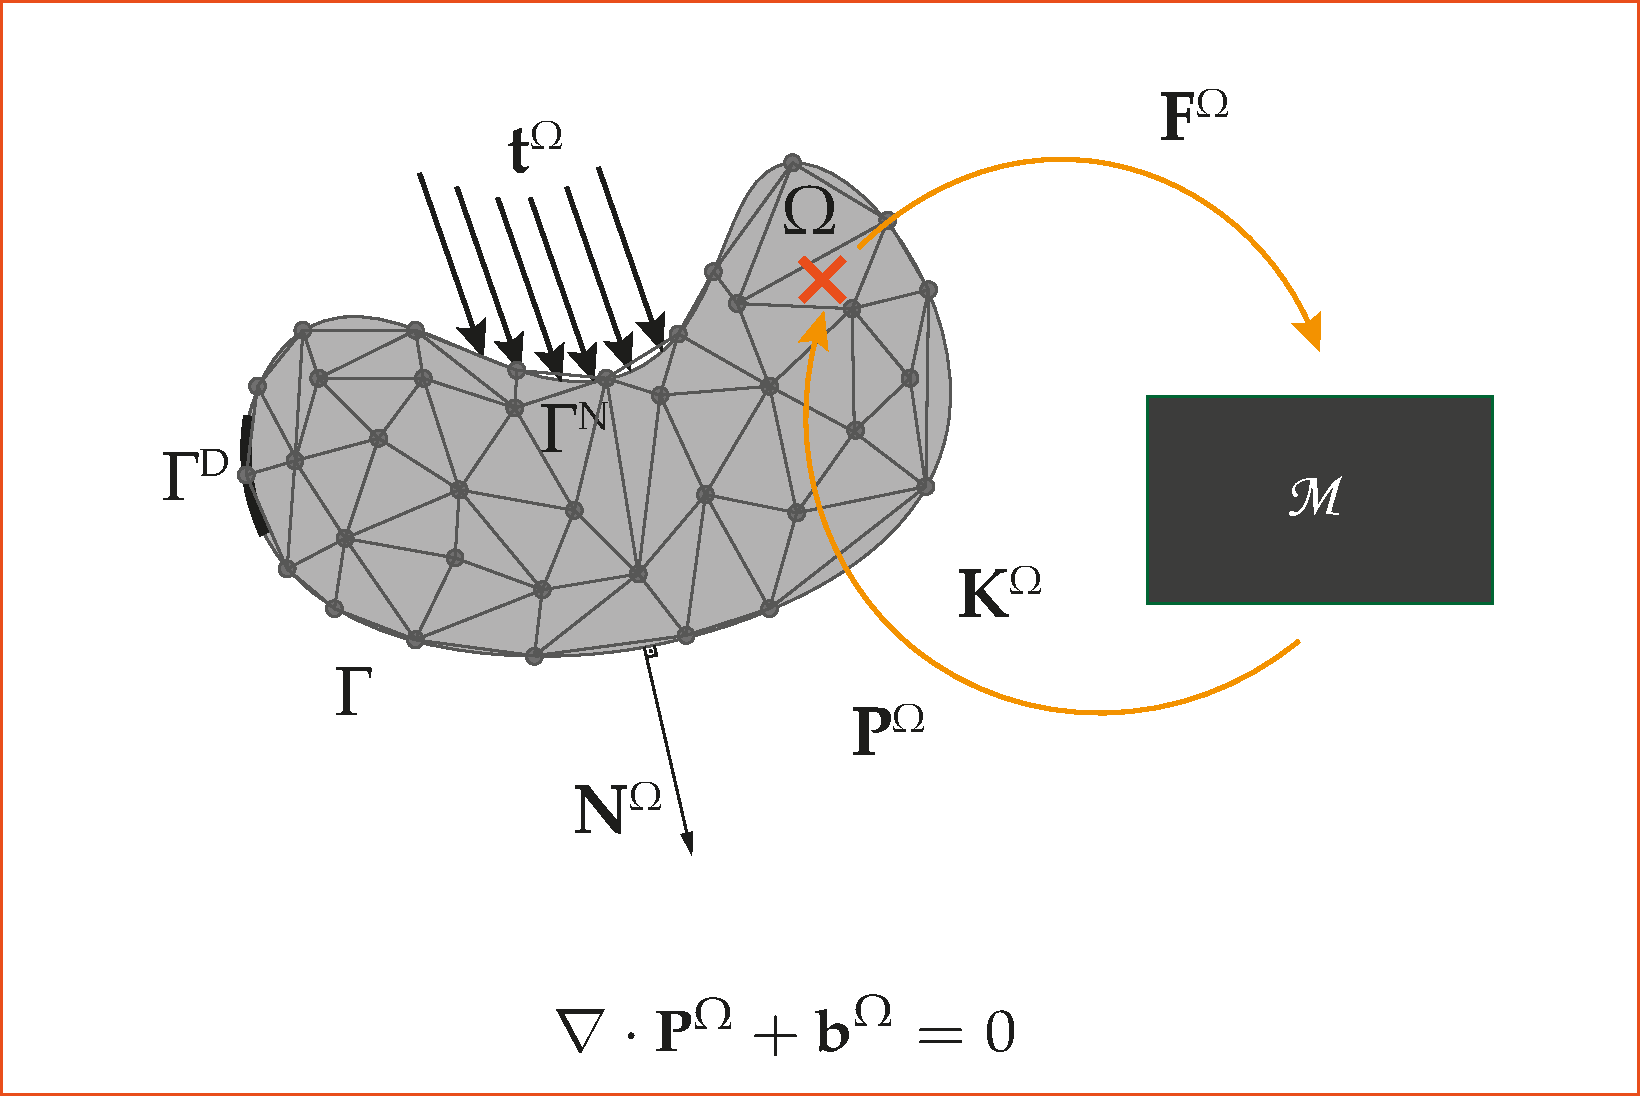
\includegraphics[width=\textwidth]{Figures/literature/FE2-ML.pdf}
  \end{minipage}%
  \begin{minipage}{0.5\textwidth} 
    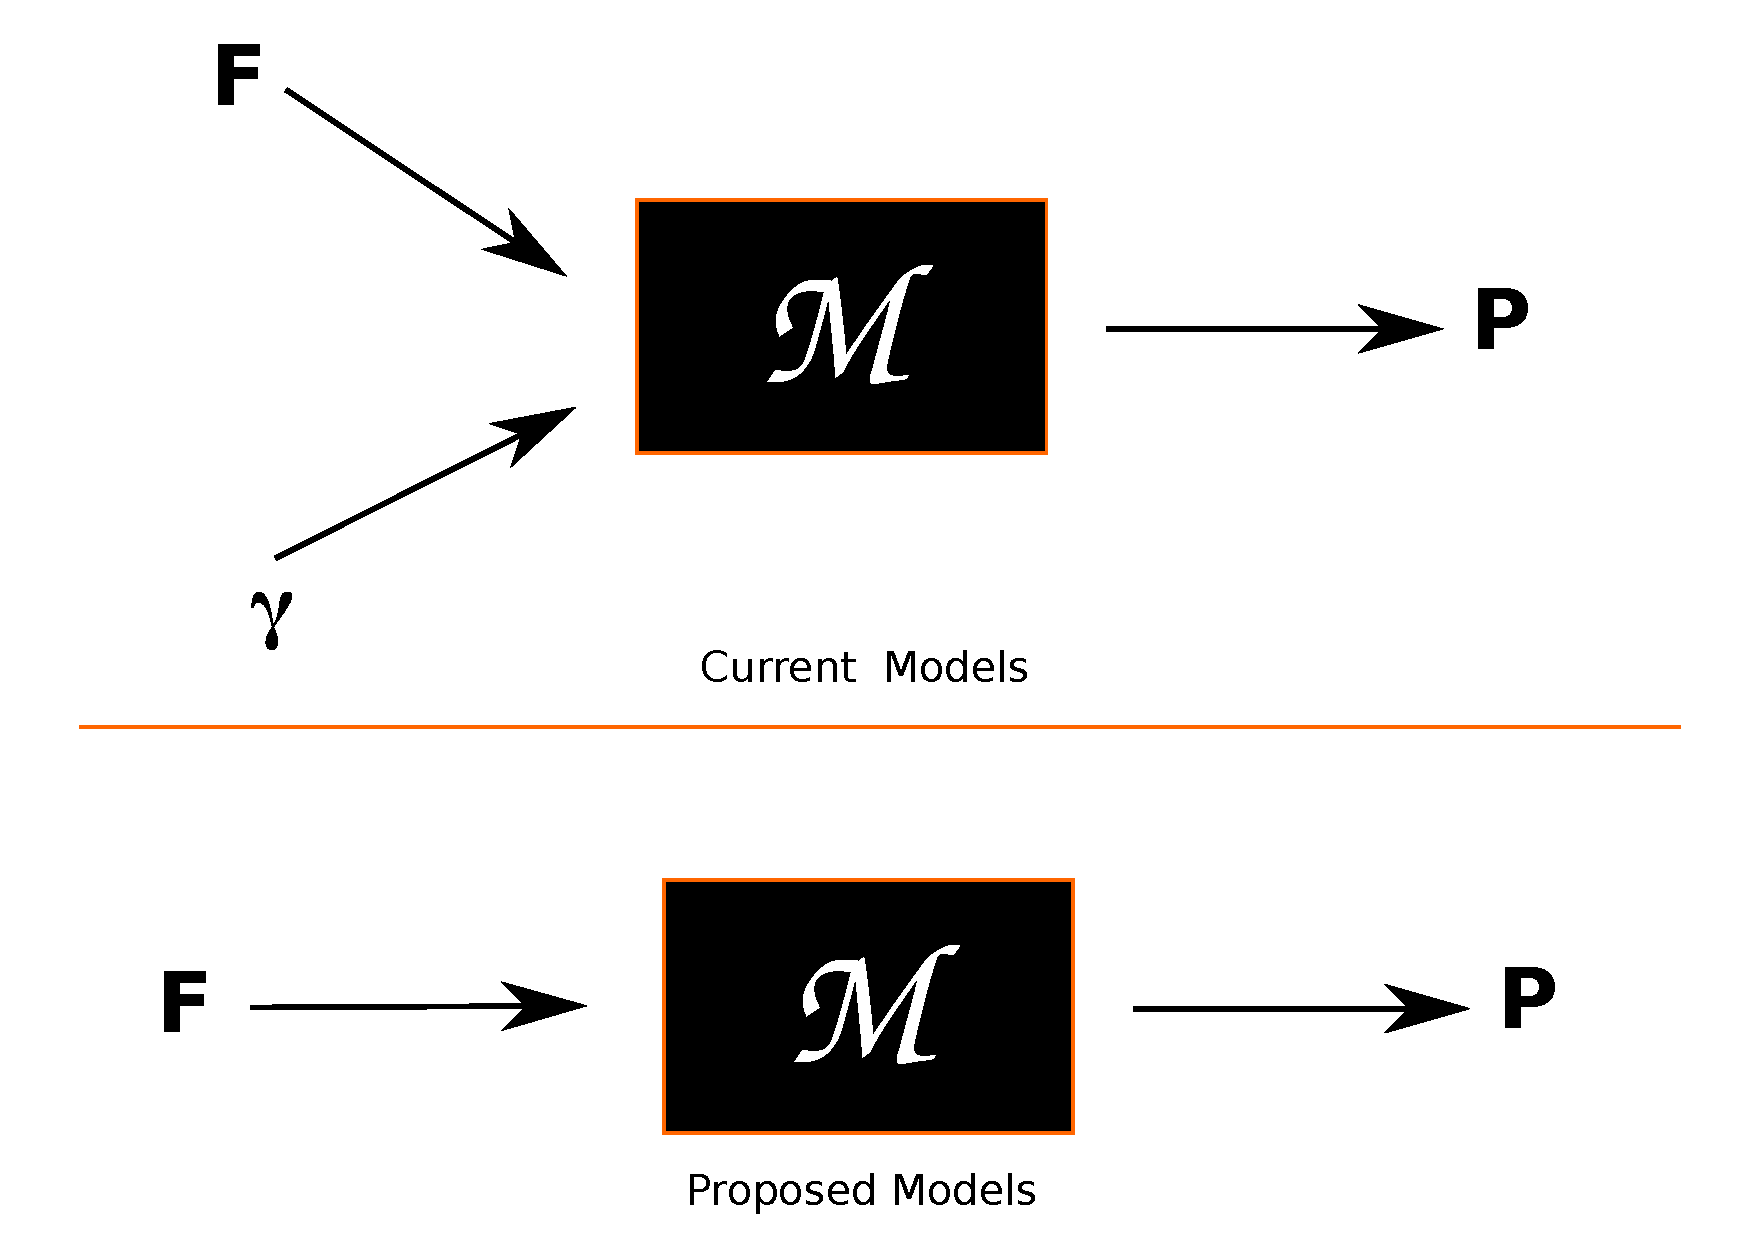
\includegraphics[width=\textwidth]{Figures/problem/models.pdf}
  \end{minipage}
}
\only<2>
{
  \begin{minipage}{0.3\textwidth} 
    \centering
    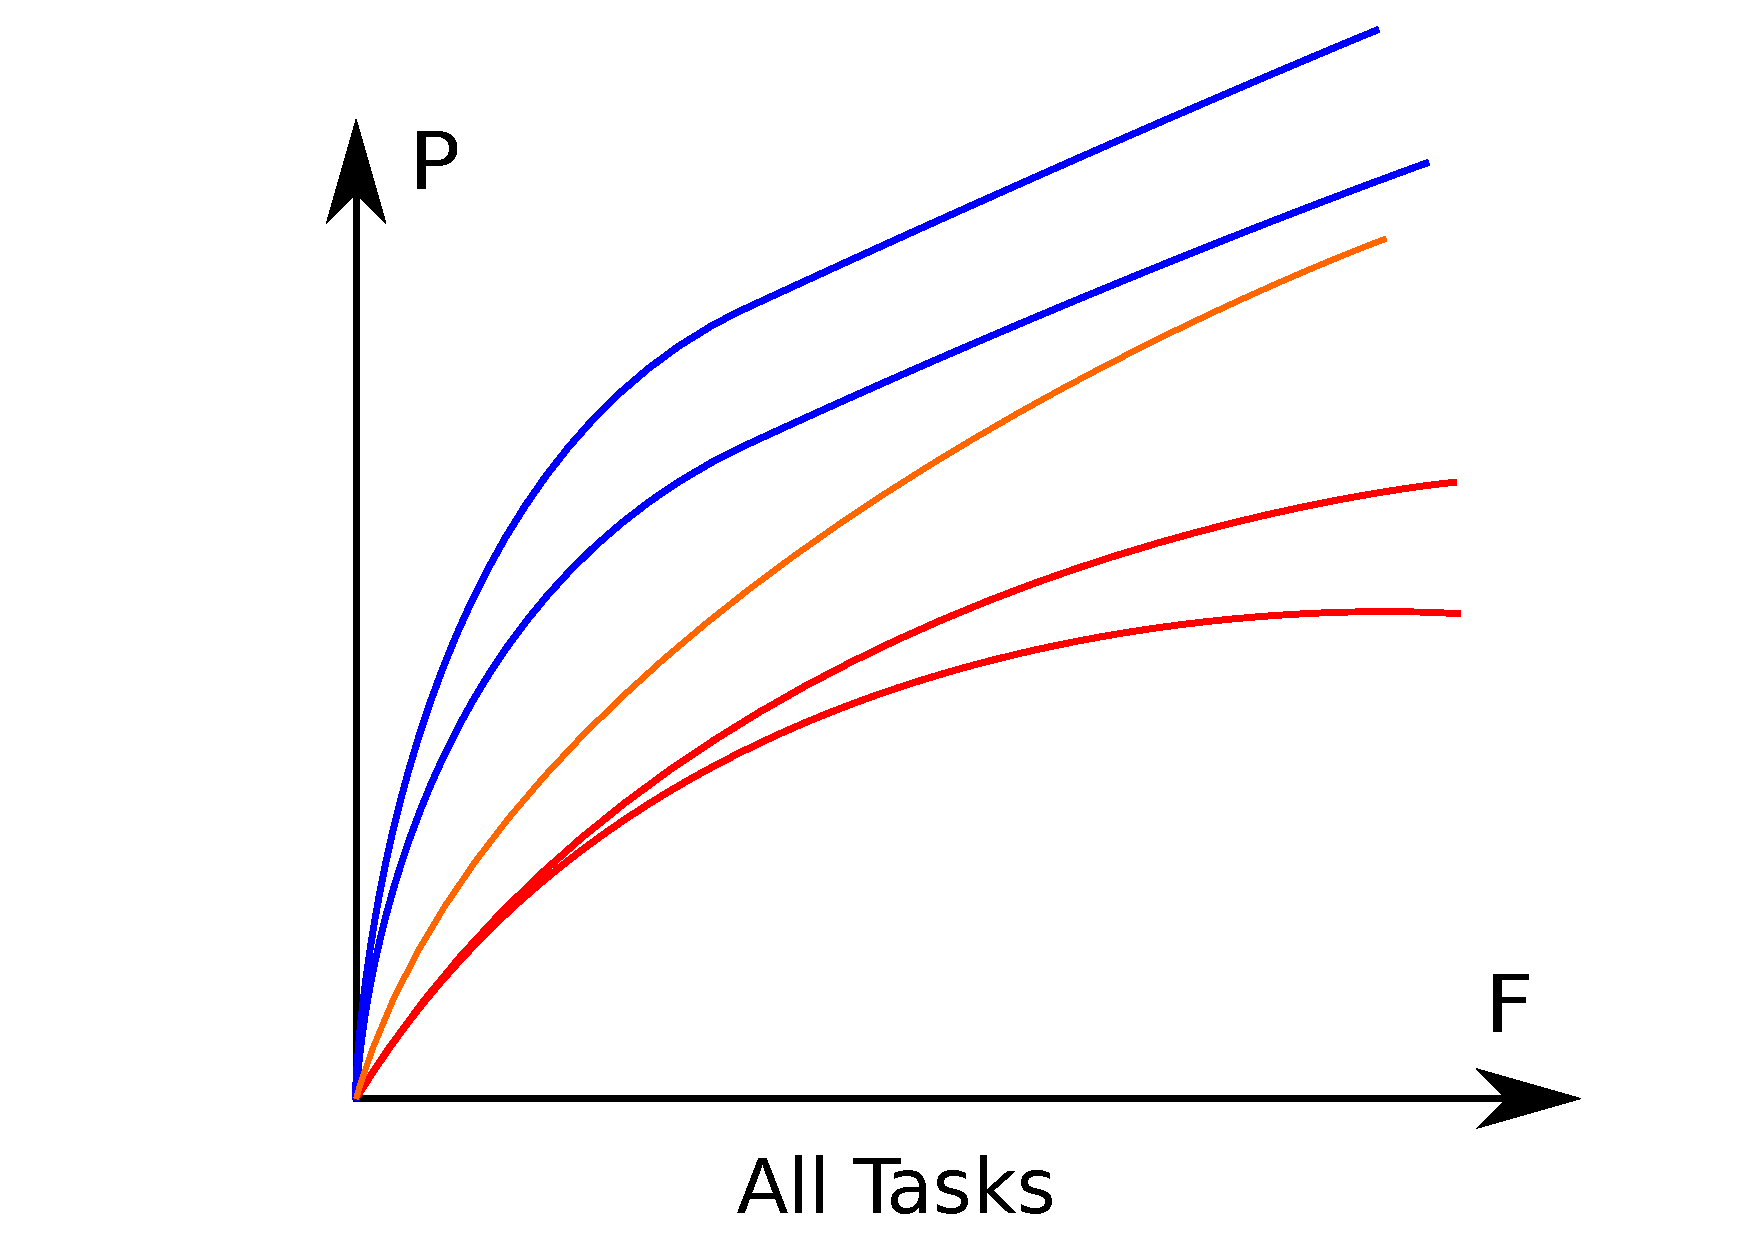
\includegraphics[width=\textwidth]{Figures/problem/collective.pdf}
  \end{minipage}%
  \begin{minipage}{0.7\textwidth} 
    \centering
    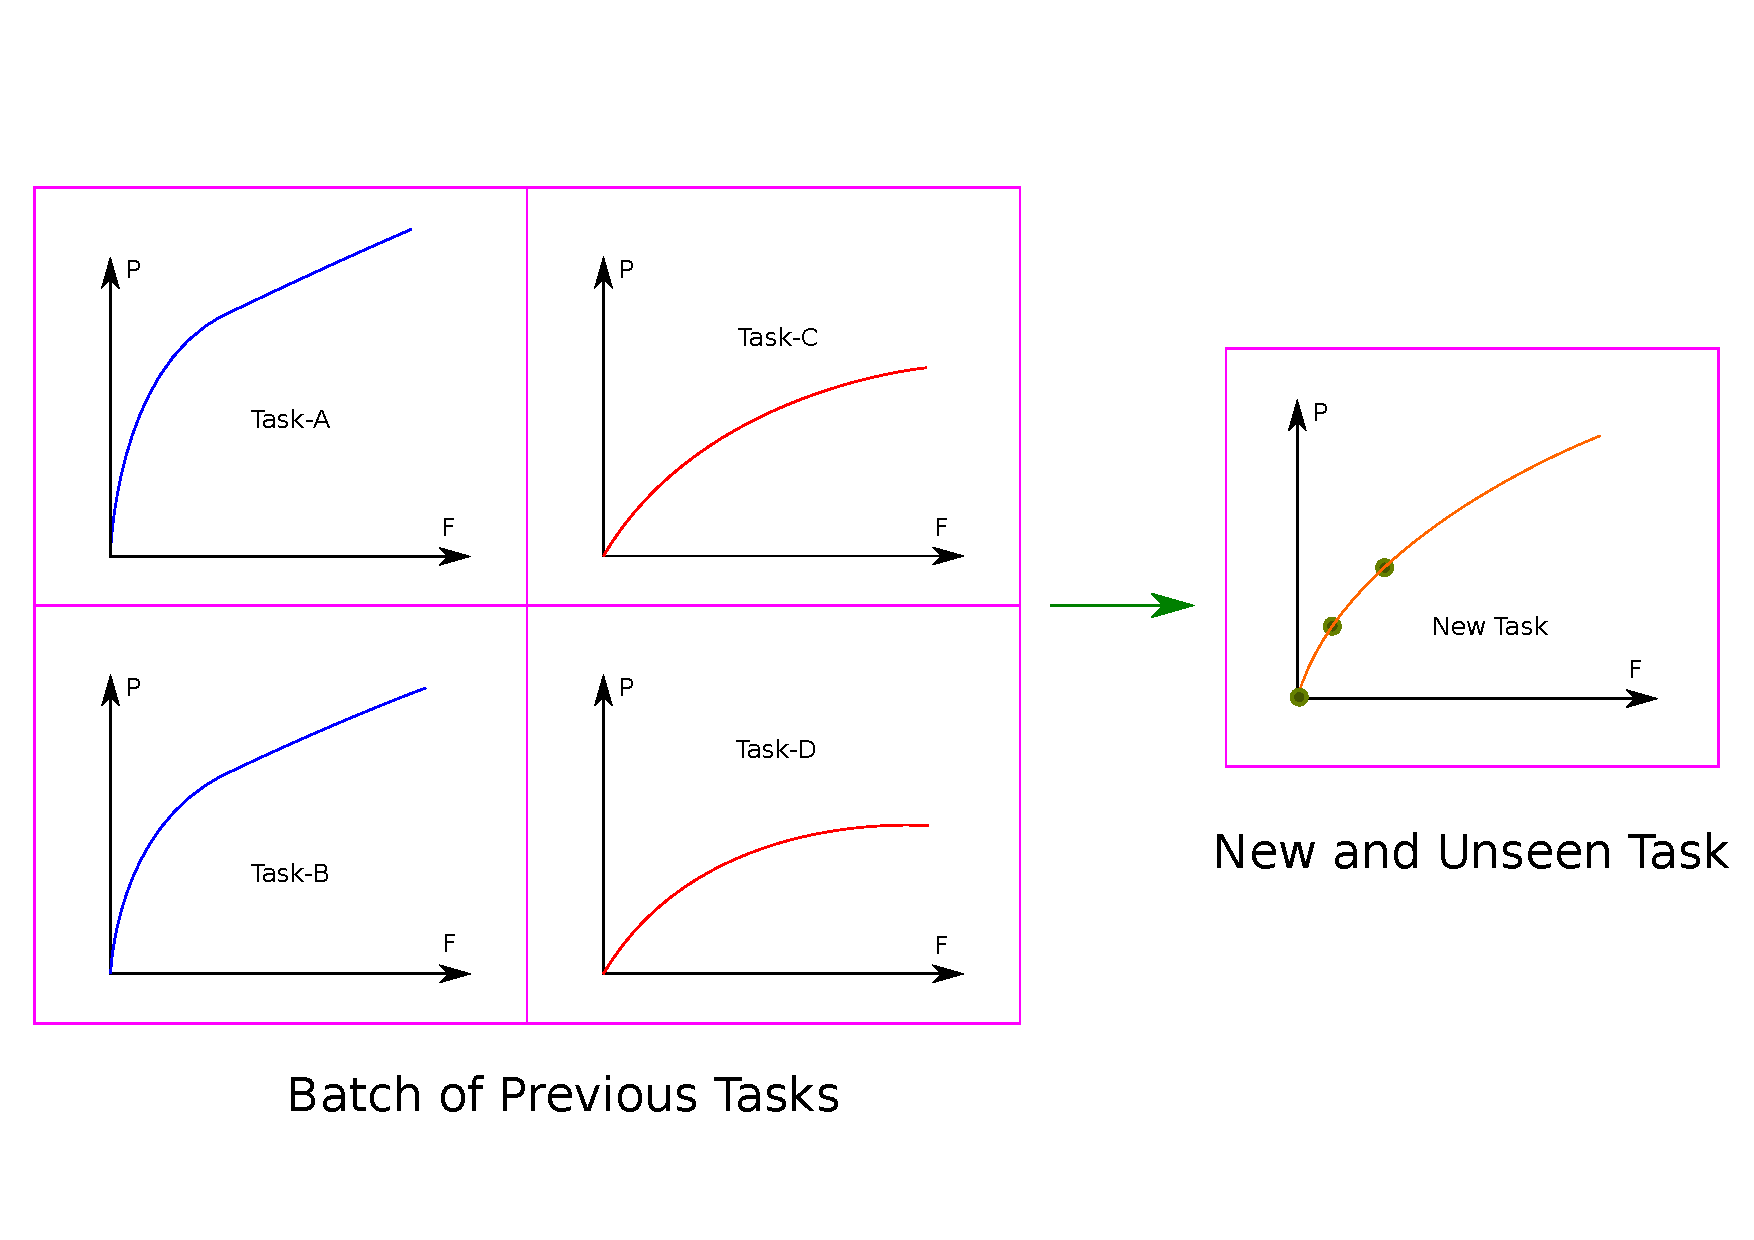
\includegraphics[width=\textwidth]{Figures/problem/material.pdf}
  \end{minipage}
}
\end{frame}

\begin{frame}{Overall Learning Problem-\only<1>{A}\only<2>{B}}
  \only<1>
{
  \color{Pink} Consider an arbitrary space that represents overall material behaviour, and the subsets of this space representing specific material types.
  \centering
  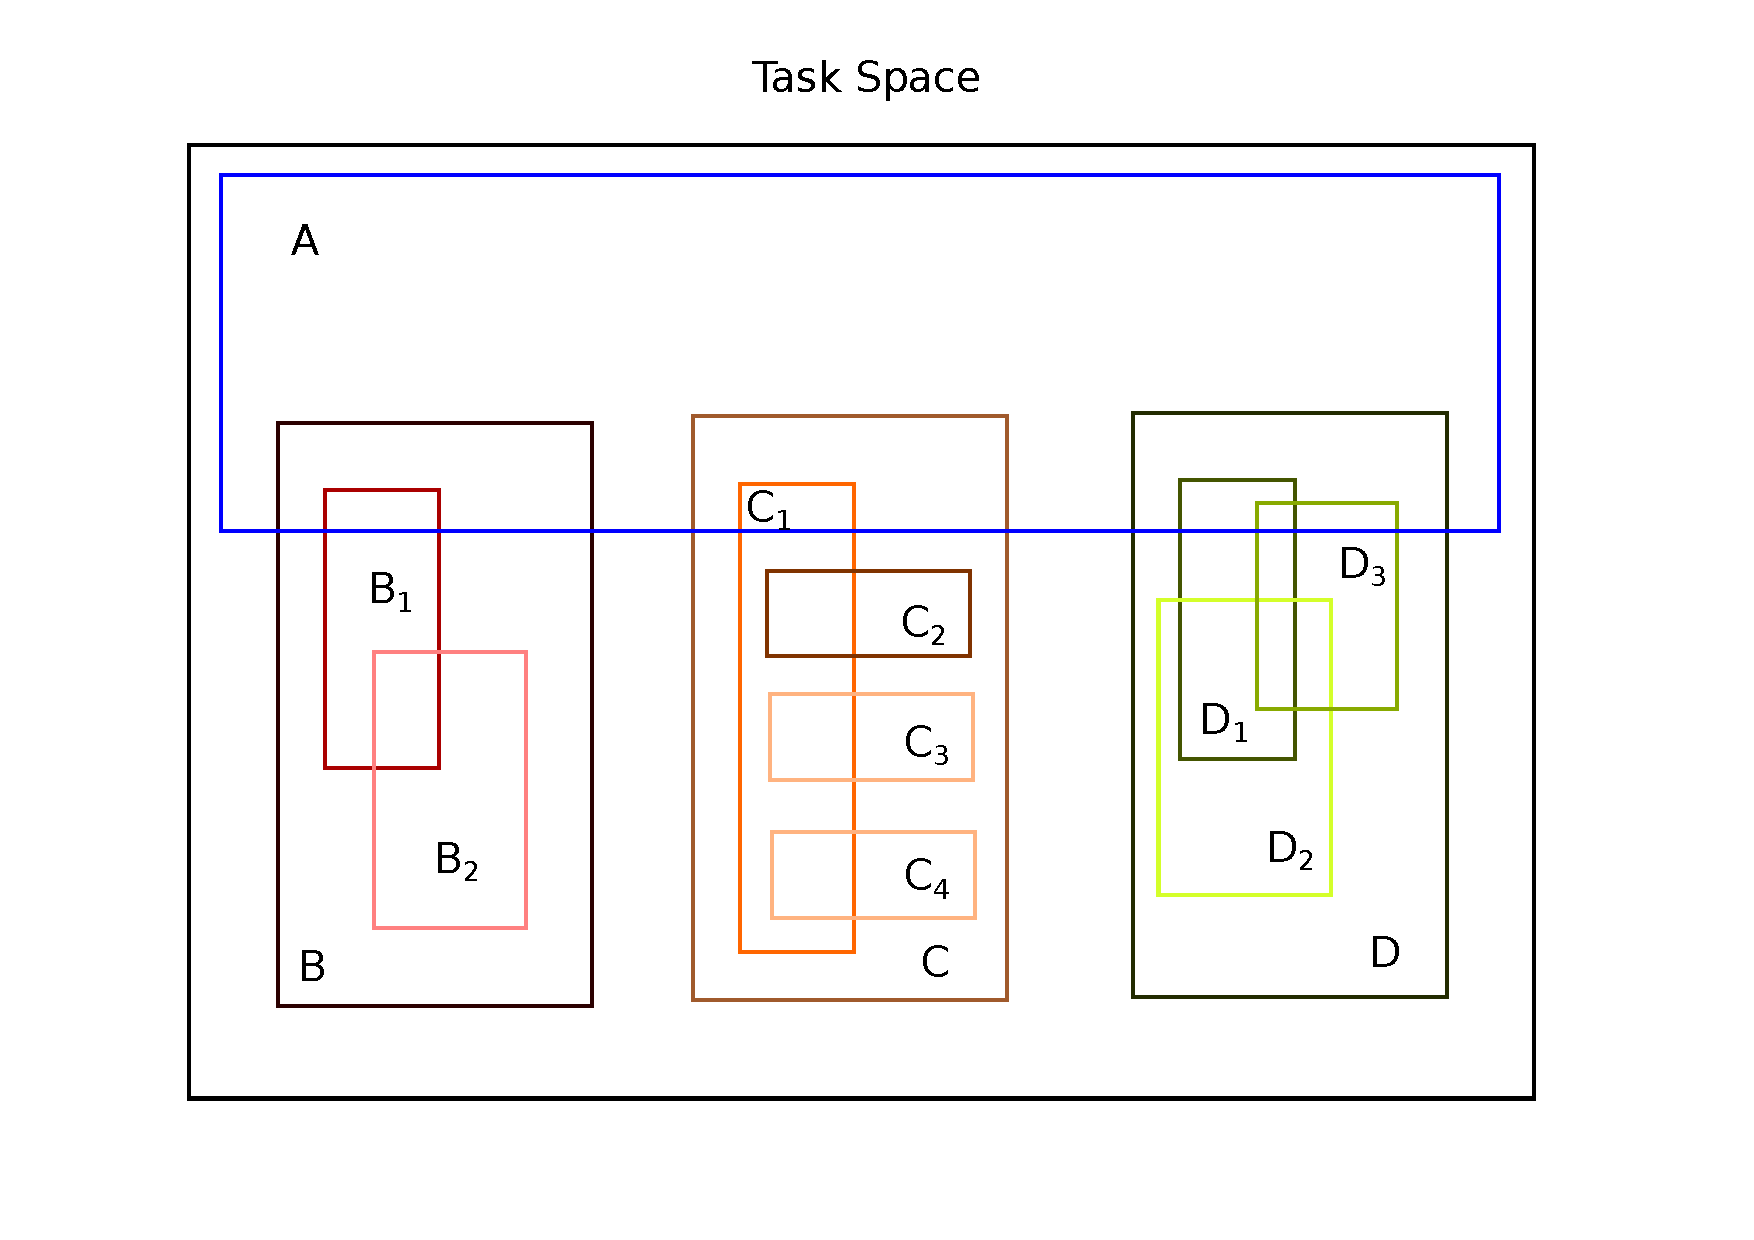
\includegraphics[width=0.6\textwidth]{Figures/problem/tasks}
}
  \only<2>
{
  \centering
  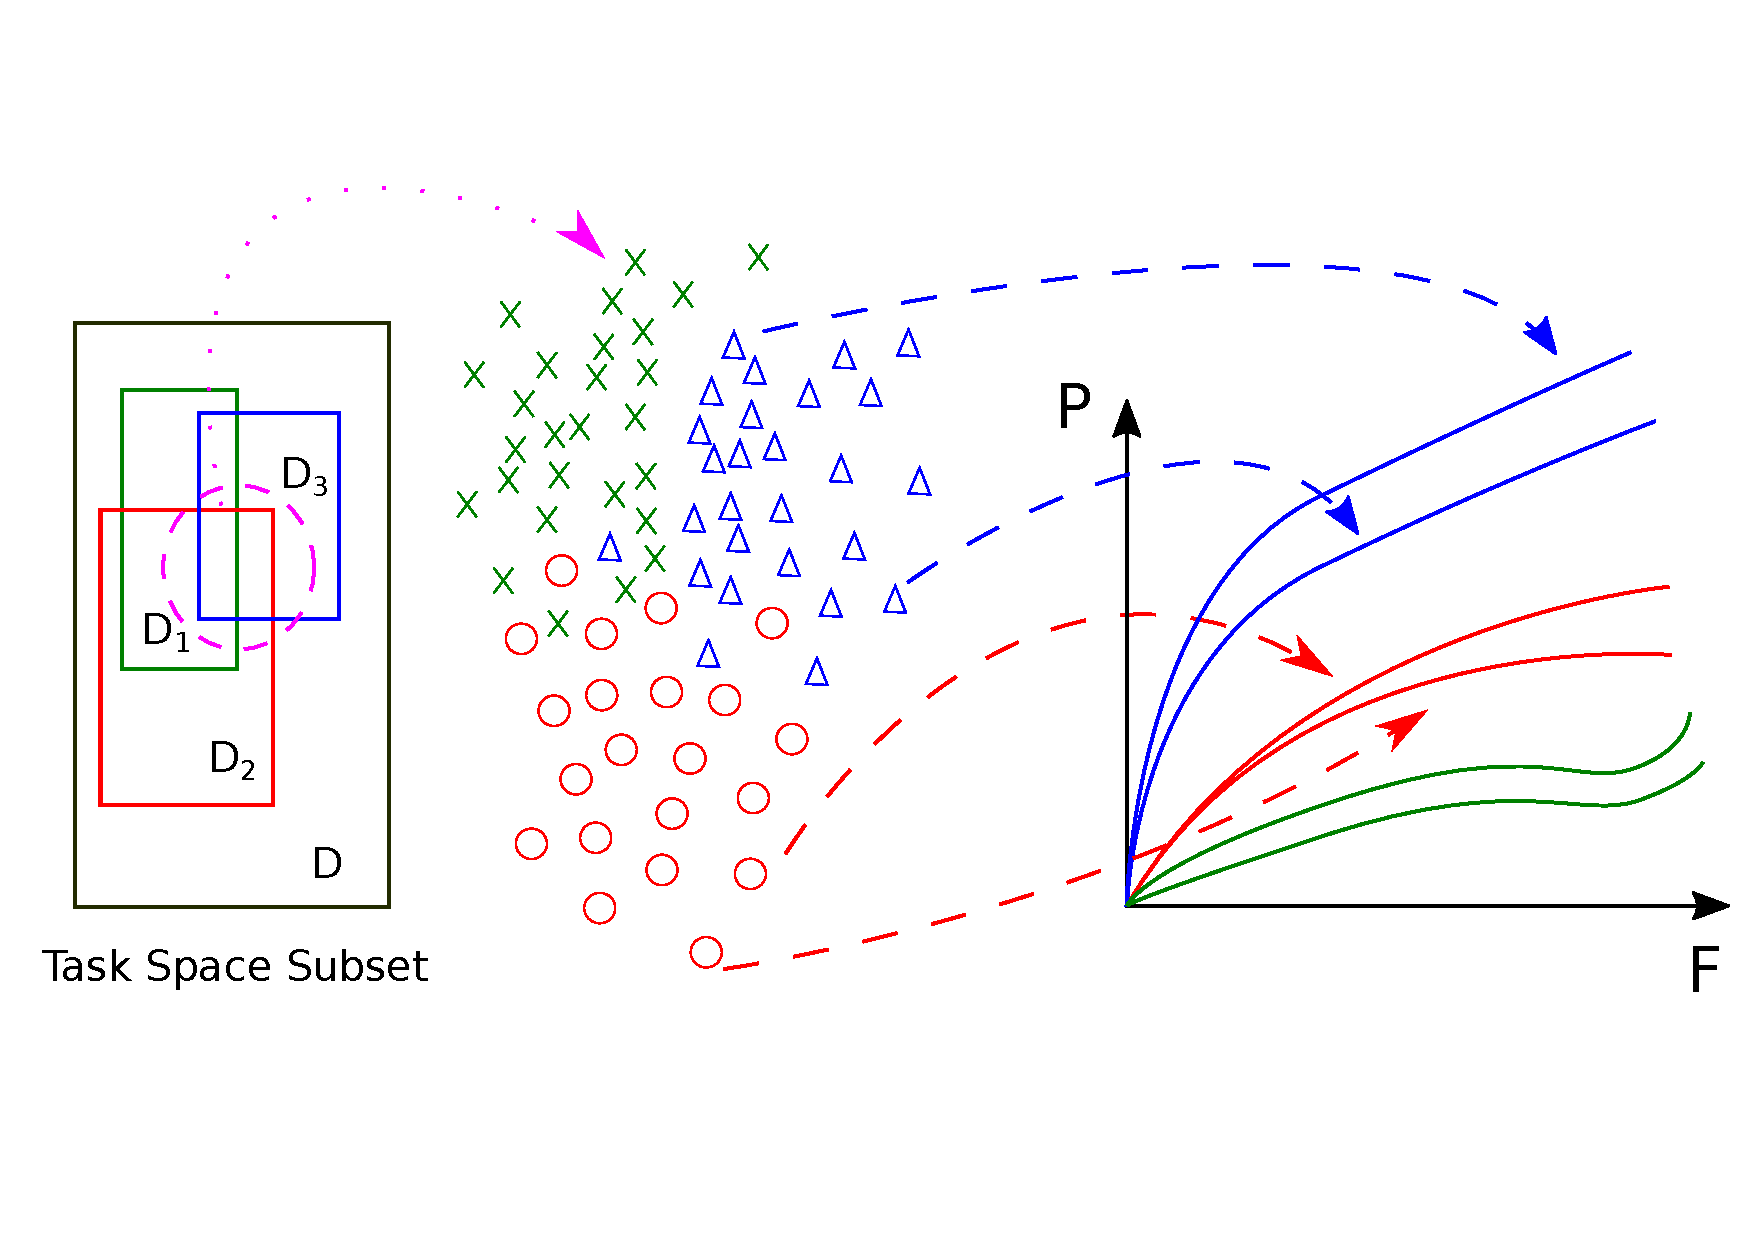
\includegraphics[width=0.5\textwidth]{Figures/problem/tasks_example}

  \begin{itemize}
  \item \color{Pink} Every label in this space becomes a full mapping! ( $T_{D_1}:=\{T_{{D_1}_i}:\mathbf{F}\to\mathbf{P}_i\}_{i=1}^M$)
  \end{itemize}
}
\end{frame}


